\scanpage{10}
\mspage{7}
We also have the homomorphism $\Lambda$ of degree $-2$, defined by
\[
\left\{\quad\cdot\ \cdot\ \cdot\ \cdot\ \cdot\ \cdot\right.
\tag{6.5}
\]
\uline{Theorem} The following conditions \inserted{\figure{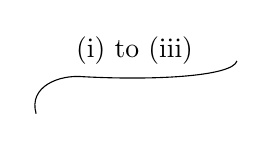
\begin{tikzpicture}[x=1cm,y=1cm]\node at (0,.35) {(i) to (iii)};\draw (-1.25,-.45) .. controls (-1.35,-.1) and (-0.95,.05) .. (-0.65,.02) .. controls (.3,-.03) and (1.25,.03) .. (1.3,.22);\end{tikzpicture}}} are equivalent

(i) The conditions \inserted{\figure{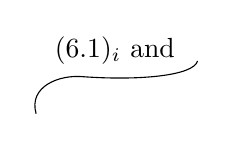
\begin{tikzpicture}[x=1cm,y=1cm]\node at (0,.35) {$(6.1)_i$ and};\draw (-1.0,-.45) .. controls (-1.1,-.1) and (-0.7,.05) .. (-0.4,.02) .. controls (.3,-.03) and (1.0,.03) .. (1.05,.22);\end{tikzpicture}}} $(6.2)_i$ for every $i$, and the $\pi_i\in\mathcal E$.

\deleted{\unsure{(ii)} [A grading of $\mathcal E^*$ can be defined by some $\pi'_i$, and for one \deleted{\illegible{2}} such choice;]\par
\unsure{(ii)} \unsure{The conditions} $(6.3)_i$ for every $i$ (with $\pi_i$ \unsure{replaced by} $\pi'_i$,....)}
\margin{\figure{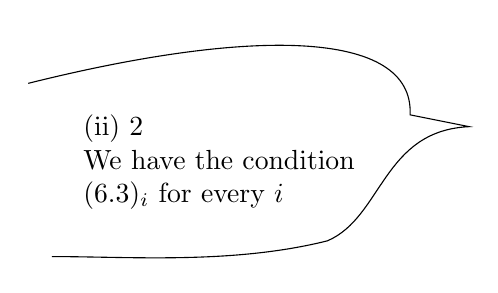
\begin{tikzpicture}[x=1cm,y=1cm]
\node[align=left,text width=4.2cm] at (0,0) {(ii) \deleted{\illegible{2}}\\We have the condition\\$(6.3)_i$ for every $i$};
\draw (-2.8,1) .. controls (0,1.7) and (2.1,1.7) .. (2.05,.6) -- (2.8,.45) .. controls (1.7,.4) and (1.7,-.7) .. (1,-1) .. controls (-.2,-1.3) and (-1.5,-1.2) .. (-2.5,-1.2);
\end{tikzpicture}}}

(iii) \deleted{The homomorphism}\inserted{We have} \inserted{\figure{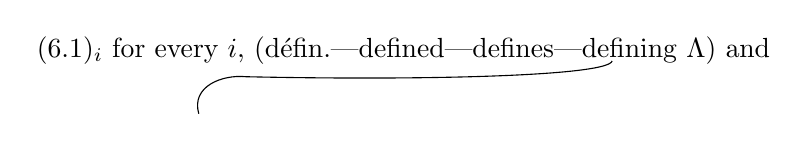
\begin{tikzpicture}[x=1cm,y=1cm]\node at (0,.35) {$(6.1)_i$ for every $i$, (\unsure{défin.|defined|defines|defining} $\Lambda$) and};\draw (-2.6,-.45) .. controls (-2.7,-.1) and (-2.3000000000000003,.05) .. (-2.0,.02) .. controls (.3,-.03) and (2.6,.03) .. (2.65,.22);\end{tikzpicture}}}
\[
\uline{\Lambda\in\mathcal E^{(-2)}}
\tag{6.6}
\]
\deleted{\unsure{(iv)}} These conditions imply in addition

(iv) The $\pi_{i,\alpha}$ are in $\mathcal E$, \deleted{the $\pi_i$ are in $\mathcal E$.}

(v) The $\pi_i\in\mathcal E$, \inserted{\figure{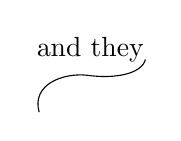
\begin{tikzpicture}[x=1cm,y=1cm]\node at (0,.35) {and they};\draw (-0.65,-.45) .. controls (-0.75,-.1) and (-0.35000000000000003,.05) .. (-0.050000000000000044,.02) .. controls (.3,-.03) and (0.65,.03) .. (0.7000000000000001,.22);\end{tikzpicture}}} are \deleted{the only projectors}\inserted{defined as forming \inserted{\figure{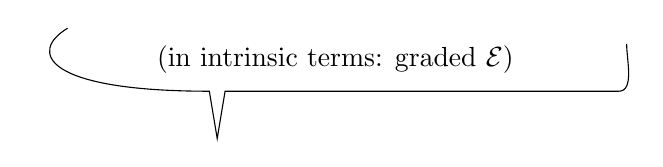
\begin{tikzpicture}[x=1cm,y=1cm]
\node at (0,.3) {(in intrinsic terms: graded $\mathcal E$)};
\draw (-3.4,.7) .. controls (-3.9,.4) and (-3.7,-.1) .. (-1.6,-.1) -- (-1.5,-.7) -- (-1.4,-.1) -- (3.6,-.1) .. controls (3.8,-.1) and (3.7,.3) .. (3.7,.5);
\end{tikzpicture}}}} the only family of elements of $\mathcal E$ satisfying $(1.1.)$ and $(1.3)$ (a) or b), as desired...., \unsure{$\mathcal E$|\deleted{$\mathcal E$}} or else $(1.4)$....).

\deleted{(vi) The element $\Lambda$ of $\mathcal E^{(-2)}$ is uniquely determined, \deleted{\unsure{by the}} (in terms of \inserted{\figure{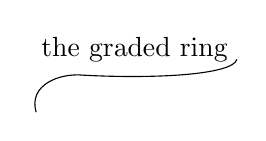
\begin{tikzpicture}[x=1cm,y=1cm]\node at (0,.35) {the graded ring};\draw (-1.25,-.45) .. controls (-1.35,-.1) and (-0.95,.05) .. (-0.65,.02) .. controls (.3,-.03) and (1.25,.03) .. (1.3,.22);\end{tikzpicture}}} $\mathcal E^*$ and the element $L\in\mathcal E^{(1)}$, by the following conditions :
\[
\left\{\begin{aligned}
L\Lambda&=1-\sum_{0\leq i\leq n}\pi_{i,0}\\
\Lambda L&=1-\sum_{n\leq i\leq2n}\pi_{i,0}
\end{aligned}\right.
\tag{6.7}
\]}

\uline{Proof.} The equivalence of (i) and (ii) is clear, and the fact that i is implied by (iii) (taking $w_i=\Lambda^{\unsure{(}n-i\unsure{)}}$). \deleted{\unsure{It}}\inserted{\figure{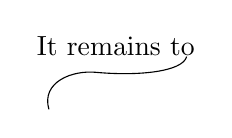
\begin{tikzpicture}[x=1cm,y=1cm]\node at (0,.35) {It remains to};\draw (-0.85,-.45) .. controls (-0.95,-.1) and (-0.55,.05) .. (-0.25,.02) .. controls (.3,-.03) and (0.85,.03) .. (0.9,.22);\end{tikzpicture}}} prove that (i), (ii) imply (iii) to (vi). We \deleted{already know}\inserted{have already indicated} that this implies \deleted{$(6.7)$} (v).
\mspage{9}
